
\documentclass[foo.tex]{subfiles}
\begin{document}

\section{Predicted SN Ia Rates}
\label{sec:predictions}

% fig 2
\begin{figure*}
\centering
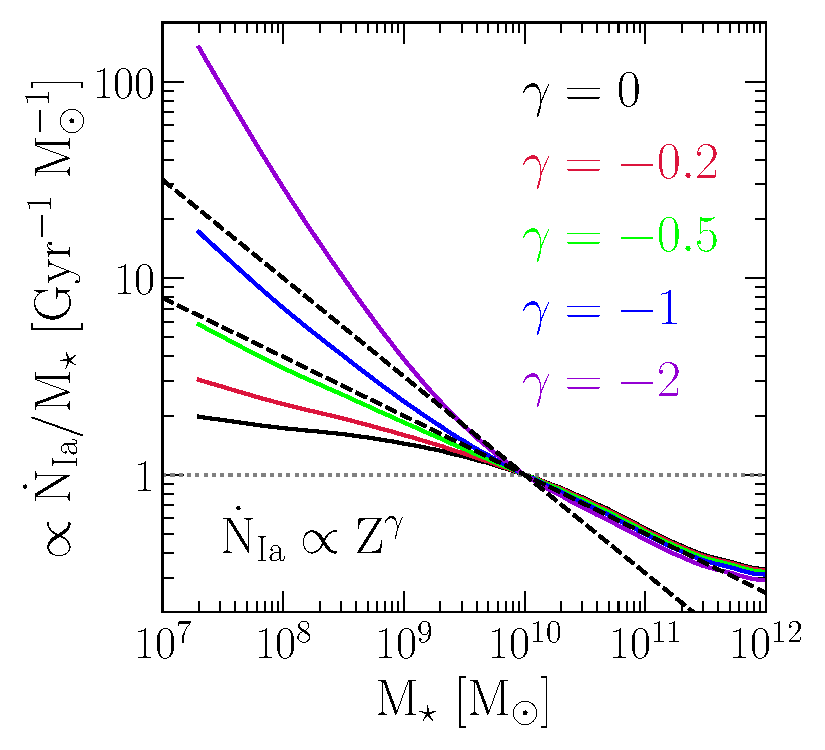
\includegraphics[scale = 0.60]{umachine_iarate_metdep.pdf}
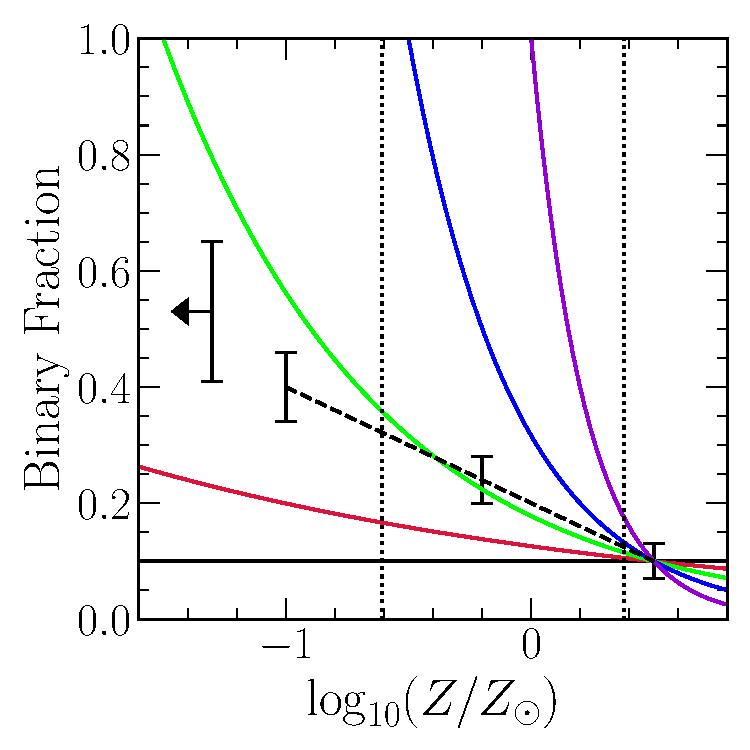
\includegraphics[scale = 0.61]{binaries_zscaling.pdf}
\caption{
\textbf{Left}: Predicted scalings of the specific SN Ia rate with galaxy
stellar mass (see equation~\ref{eq:specia}) assuming the mean~\um~SFHs and a
single power-law~$Z^\gamma$ metallicity-dependence with~$\gamma = 0$ (i.e. no
dependence; black),~$\gamma = -0.2$ (red), $\gamma = -0.5$ (green),
$\gamma = -1$ (blue), and~$\gamma = -2$ (purple).
Following~\citet{Brown2019} and~\citet{Gandhi2022}, we normalize all rates to
a value of 1 at~$\mstar = 10^{10}~\msun$.
Black dashed lines denote the scalings of~$\dot{\text{N}}_\text{Ia} / \mstar
\sim \mstar^{-0.5}$ and~$\dot{\text{N}}_\text{Ia} / \mstar \sim \mstar^{-0.3}$
derived when normalizing the observed rates by the~\citet{Bell2003} and
\citet{Baldry2012} SMFs, respectively.
\textbf{Right}: The same metallicity scalings as in the left panel in
comparison to the close binary fractions observed in APOGEE
\citep[][black dashed line with error bars]{Moe2019} normalized to the observed
binary fraction of 10\% at~$\log_{10}(Z / Z_\odot) = +0.5$.
The characteristic metallicities of~$\mstar = 10^{7.2}~\msun$
($\log_{10}(Z / Z_\odot) \approx -0.6$) and~$10^{10}~\msun$ galaxies 
($\log_{10}(Z / Z_\odot) \approx +0.4$) are marked with black dotted lines.
The arrow denotes the binary fraction of 53\%~$\pm$ 12\% measured by
\citet{Moe2019} at [Fe/H] = $-3$.
}
\label{fig:specia_metdep}
\end{figure*}

% fig 3
\begin{figure*}
\centering
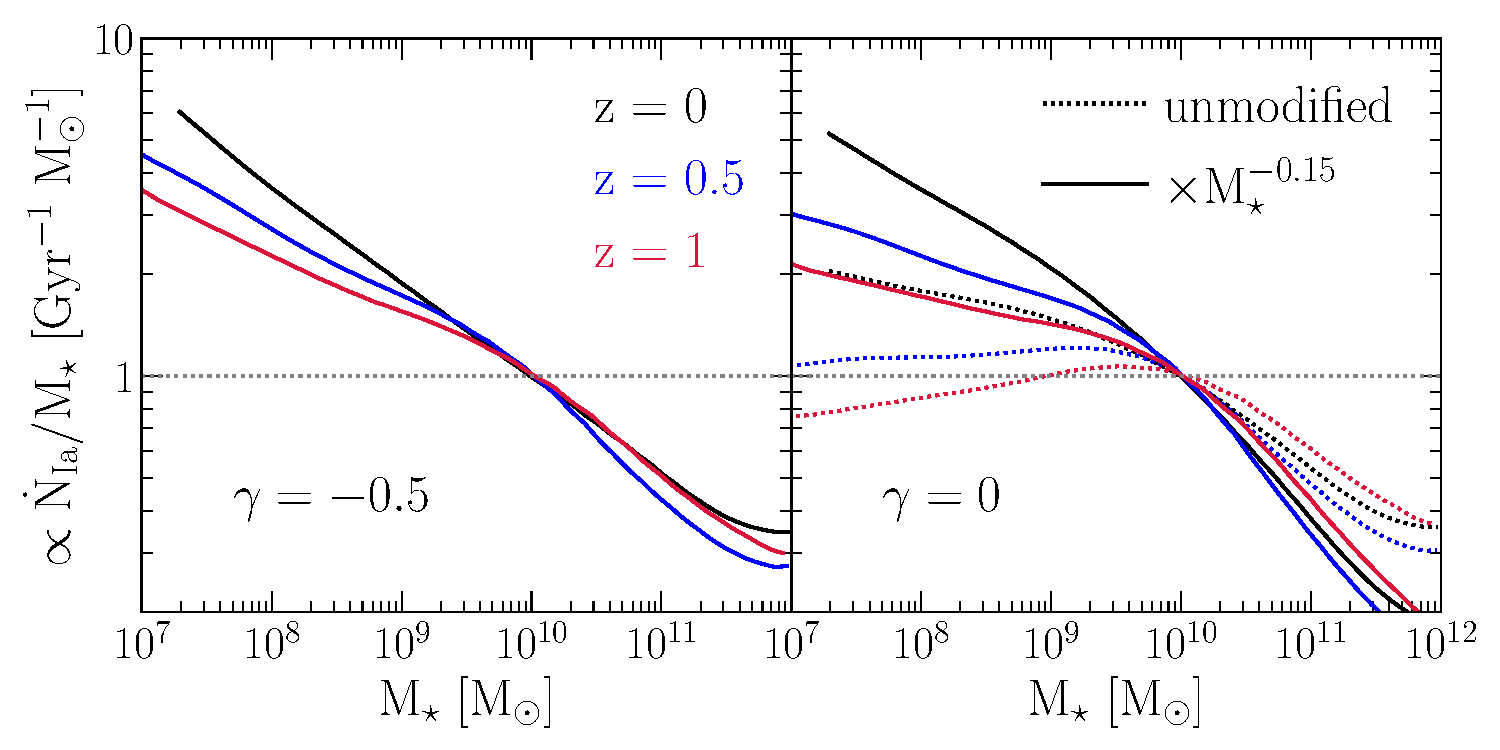
\includegraphics[scale = 0.65]{umachine_iarate_redshiftevol.pdf}
\caption{
The specific SN Ia rate normalized to~$1$ at~$10^{10}~\msun$ as a function of
stellar mass with ($\gamma = -0.5$, left) and without a metallicity dependence
($\gamma = 0$, right) at redshifts $z = 0$ (black),~$z = 0.5$ (blue),
and~$z = 1$ (red).
In the right panel, we artificially scale the rates by a factor of
$(\mstar / 10^{10}~\msun)^{-0.15}$ to bring the~$z = 0$ predictions into
better agreement with an~$\sim \mstar^{-0.3}$ scaling as predicted by the
$\gamma = -0.5$ case.
Stellar masses correspond to the appropriate redshift (i.e., the rates for
$z = 1$ use the~$z = 1$ stellar masses and not the present-day stellar
masses).
We show the unmodified rates as dotted lines (the black solid line in the left
panel and the black dotted line in the right panel are the same as the green
line and black solid line in the left panel of Fig.~\ref{fig:specia_metdep}).
}
\label{fig:specia_zdep}
\end{figure*}

The left panel of Fig.~\ref{fig:specia_metdep} shows the specific SN Ia rate
for several choices of~$\gamma$ in comparison to the~$\dot{\text{N}}_\text{Ia} /
\mstar \sim \mstar^{-0.5}$ and~$\dot{\text{N}}_\text{Ia} / \mstar \sim
\mstar^{-0.3}$ scalings of the observed rate with the~\citet{Bell2003} and
\citet{Baldry2012} SMFS, respectively.
The metallicity dependence has a significant impact only below
$\mstar \approx 3\times10^9~\msun$ due to the shape of the MZR;
this is the mass above which the MZR flattens considerably (see
Fig.~\ref{fig:sfh_mzr}).
Assuming no metallicity dependence (i.e.~$\gamma = 0$), these calculations
suggest that the variations in SFHs between~$\sim$$10^{7.2}$ and
$\sim$$10^{10}~\msun$ can account for only a factor of~$\sim$2 increase in the
specific SN Ia rate.
The~$\gamma = -0.5$ case is generally consistent with a mass dependence
of~$\mstar^{-0.3}$, while the steeper dependence of~$\mstar^{-0.5}$ would
require a stronger scaling of roughly~$\gamma \approx -1.5$.
% \citet{Gandhi2022} advocate for a~$\gamma \approx -0.5$ scaling, additionally
% demonstrating that incorporating this metallicity dependence into the
% FIRE-2\footnote{
% 	Feedback In Realistic Environments.
% 	\url{https://fire.northwestern.edu/}
% } cosmological zoom-in simulations~\citep{Hopkins2018} leads to better
% agreement with the stellar masses and iron abundances measured by
% \citet{Gallazzi2005} and~\citet{Kirby2013}.
\par
In the right panel of Fig.~\ref{fig:specia_metdep}, we compare the same
scalings to the close binary fractions in APOGEE measured by~\citet{Moe2019}.
{\color{red}
The binary fraction must eventually saturate, along with its impact on SN
rates, and~\citet{Moe2019} measured
$53 \pm 12$\% in the most metal-poor stars ([Fe/H]~$\approx -3$), which we
also include in Fig.~\ref{fig:specia_metdep}.
However, our sample does not extend to such low metallicities.
% We have additionally marked~\citeauthor{Moe2019}'s~\citeyearpar{Moe2019}
% measurement of the binary fraction in the most metal-poor stars
% ([Fe/H]~$\approx -3$), a point above which one would naturally expect the
% metallicity dependence of the SN Ia rate to flatten off if binarity is the
% primary driver.
}
The line at~$Z \approx 10^{-0.6} Z_\odot$ is the characteristic abundance of
an~$\mstar = 10^{7.2}~\msun$ galaxy in the~\citet{Zahid2014} parametrization.
For the range of metallicities spanned by the stellar masses we explore here,
the close binary fraction is remarkably consistent with a~$\gamma = -0.5$
scaling with metallicity.
% If the~$\sim$$\mstar^{-0.3}$ scaling found by~\citet{Gandhi2022} is accurate,
% then this result suggests that the increase of the specific SN Ia rate with
% decreasing stellar mass can be explained entirely by dwarf galaxies having more
% extended SFHs and a higher close binary fraction due to their lower abundances.
If one instead takes~$Z \approx 0.1Z_\odot$ for a~$\sim$$10^{7.2}~\msun$ galaxy
as suggested by~\citet{Andrews2013}, then there is a slight tension between a
$\gamma = -0.5$ scaling and the close binary fraction measured by
\citet{Moe2019}.
{\color{red}
That is, although the normalization of the MZR does not impact our predicted
scaling of the specific SN Ia rate with stellar mass, it does impact whether or
not binarity can explain the effect across the full range of metallicities.
In particular, the stellar MZR has a lower normalization
\citep[e.g.,][]{Gallazzi2005, Kirby2013, Simon2019}, reaching [Fe/H]~$\approx
-1$ at~$\sim$$2\times10^8 \msun$.
Comparing this normalization with~\citeauthor{Moe2019}'s~\citeyearpar{Moe2019}
measurement at [Fe/H]~$\approx -3$ suggests that variations in binarity may be
minimal in the~$10^7 - 10^8~\msun$ range and that additional effects would be
required to explain a steep increase in SN Ia rates with decreasing mass.
}
% {\color{red}
% We have additionally marked~\citeauthor{Moe2019}'s~\citeyearpar{Moe2019}
% measurement of the binary fraction in the most metal-poor stars
% ([Fe/H]~$\approx -3$), a point above which one would naturally expect the
% metallicity dependence of the SN Ia rate to flatten off if binarity is the
% primary driver.
% We also note that the normalization of the MZR does impact whether or not this
% $Z^{-0.5}$ scaling 
% }
\par
There is some additional freedom to adjust the metallicity dependence beyond
that of binaries, so the agreement need not be perfect.
For example, any additional increase in the SN Ia rates not supplied by an
increased binary fraction could arise due to more massive WDs forming at
low~$Z$ -- the scenario postuled by~\citet{Kistler2013}.
% If both the~\citet{Andrews2013} MZR and the~$\gamma = -0.5$ scalings are
% accurate, then it would be reasonable to suggest that the additional increase
% in the SN Ia rates not supplied by the increased binary fraction arise due to
% more massive WDs forming at low~$Z$ -- the scenario postulated by
% \citet{Kistler2013}.
Nonetheless, it appears that the scaling of the close binary fraction with
metallicity can explain the majority of the effect if the rate scales with mass
as~$\dot{\text{N}}_\text{Ia} / \mstar \sim \mstar^{-0.3}$.
If, instead, the~$\sim$$\mstar^{-0.5}$ scaling found using the~\citet{Bell2003}
SMF is accurate, then the required~$\gamma \approx -1.5$ scaling cannot be
explained by the close binary fraction alone as it would reach unphysical
values ($>1$) within the range of observed metallicities.
\par
% Such scalings are disfavored by~\citet{Gandhi2022} because they fail to
% reproduce the well-known correlations between stellar [Mg/Fe] and [Fe/H]
% abundances as observed in M31 satellites by~\citep*{Vargas2014} but are still
% within the range of theoretical possibilities because only a small fraction of
% WDs actually explode ($\sim4$\% if the progenitors are~$\sim3 - 8~\msun$
% stars;~\citealp{Maoz2012b}).
% In the next section, we discuss potential observational diagnostics of
% a~$Z^{-0.5}$ metallicity dependence or lack thereof.
Due to the evolution of the MZR, the mass dependence of the specific SN Ia rate
at different redshifts could empirically distinguish between~$\gamma = 0$ and
$\gamma = -0.5$.
To investigate this possibility, we simply evaluate equation~\refp{eq:specia}
over the appropriate range of lookback times assuming standard cosmological
parameters~\citep{Planck2014}.
For the~$\gamma = 0$ case, we also show the effect of applying an additional
$(\mstar / 10^{10}~\msun)^{-0.15}$.
This prefactor brings the~$\gamma = 0$ predictions into better agreement with
the empirical~$\dot{\text{N}}_\text{Ia} / \mstar \sim \mstar^{-0.3}$ scaling
at~$z = 0$ and is intended to encapsulate the mass scaling needed for some
other unknown process to sufficiently amplify the SN Ia rate at low stellar
masses if it is instead not due to metallicity effects.
\par
We show the resulting specific SN Ia rates as a function of stellar mass at
$z = 0$,~$0.5$ and~$1$ in Fig.~\ref{fig:specia_zdep}.
In both the~$\gamma = 0$ and $\gamma = -0.5$ cases, the scaling of the specific
SN Ia rate with galaxy stellar mass becomes shallower with increasing redshift.
If~$\gamma = -0.5$, these calculations suggest that it should decrease by a
factor of~$\sim$2 between~$z = 0$ and~$z = 1$ at~$\mstar \approx
10^{7.2}~\msun$, the lowest stellar mass for which we have made predictions at
all three redshifts.
If~$\gamma = 0$, then the rate instead decreases by a factor of~$\sim$3 at
$\sim 10^{7.2}~\msun$.
This difference arises because the metallicities of dwarf galaxies decrease
with increasing redshift and~$\gamma = -0.5$ allows them to sustain higher
SN Ia rates than if~$\gamma = 0$.
Empirically, the cosmic SN Ia rate increases with redshift
\citep[e.g.][]{Graur2014}, and we have verified that our framework reproduces
this result by integrating over the SMF (similar to equation
\ref{eq:hostmassdist} below).
Given this result and the lower stellar masses of the host galaxies at high
redshift, one might expect the trend to steepen with increasing~$z$.
The slope instead decreases here because the lines in Fig.~\ref{fig:specia_zdep}
(right panel) are moving to the right with time as galaxies grow in mass, and
we normalize to unity at a stellar mass of~$10^{10}~\msun$ at all redshifts.
% Distinguishing between these models empirically, however, would require a
% considerably precise SMF at redshift~$z = 1$.
% Factors of 2 and 3 between~$10^{7.2}$ and~$10^{10}~\msun$ are produced by
% power-law indices of~$-0.108$ and~$-0.170$, respectively. 
% The difference between the two ($0.062$) is the minimum precision required
% on the slope of the SMF at the low-mass end, only slightly larger than the
% precision achieved by~\citet[][$\pm 0.05$, see their Fig. 13]{Baldry2012}.
% Therefore, this empirical test requires at least their level of precision but
% at~$z \approx 1$.
% \par
% Stellar masses can then be derived for the host galaxies which have
% spectroscopic information available from, e.g., JWST itself or the Dark Energy
% Spectroscopic Instrument~\citep[DESI;][]{Desi2016}.
% However, the resultant constraints on the specific SN Ia rate as a function of
% stellar mass will require precise nkowledge of how the SMF varies with redshift.
% Such measurements are challenging with current galaxy samples from, e.g.,
% SDSS due to their flux-limited nature and the broad range of mass-to-light
% ratios spanned by galaxies~\citep{Weigel2016}.
% State-of-the-art facilities like DESI and JWST which have recently begun
% collecting data should achieve significantly higher completeness for dwarf
% galaxies at~$z \approx 1$ due to their higher sensitivities, but as discussed
% above, achieving the level of precision required for this empirical test could
% be challenging, even with these instruments.

% fig 4
\begin{figure}
\centering
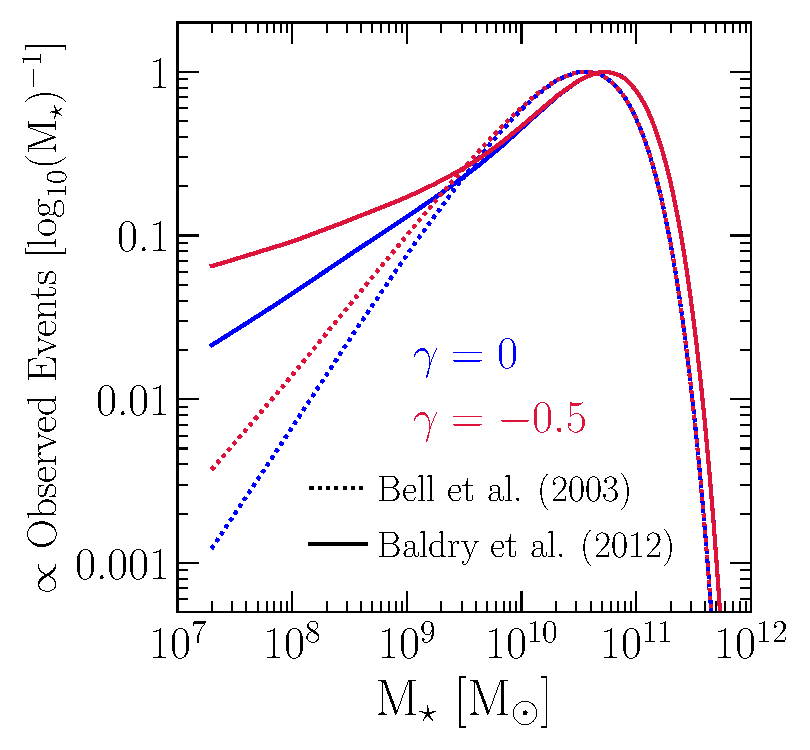
\includegraphics[scale = 0.55]{ia_massdist.pdf}
\caption{
The predicted stellar mass distribution of~$z = 0$ SN Ia host galaxies in an
untargeted survey (see equation~\ref{eq:hostmassdist}) with the
\citet[][dotted]{Bell2003} and~\citet[][solid]{Baldry2012} SMFs for both
metallicity-dependent ($\gamma = -0.5$, red) and metallicity-independent rates
($\gamma = 0$, blue).
All distributions are normalized to a maximum value of 1.
}
\label{fig:hostmassdist}
\end{figure}

% fig 5
\begin{figure*}
\centering
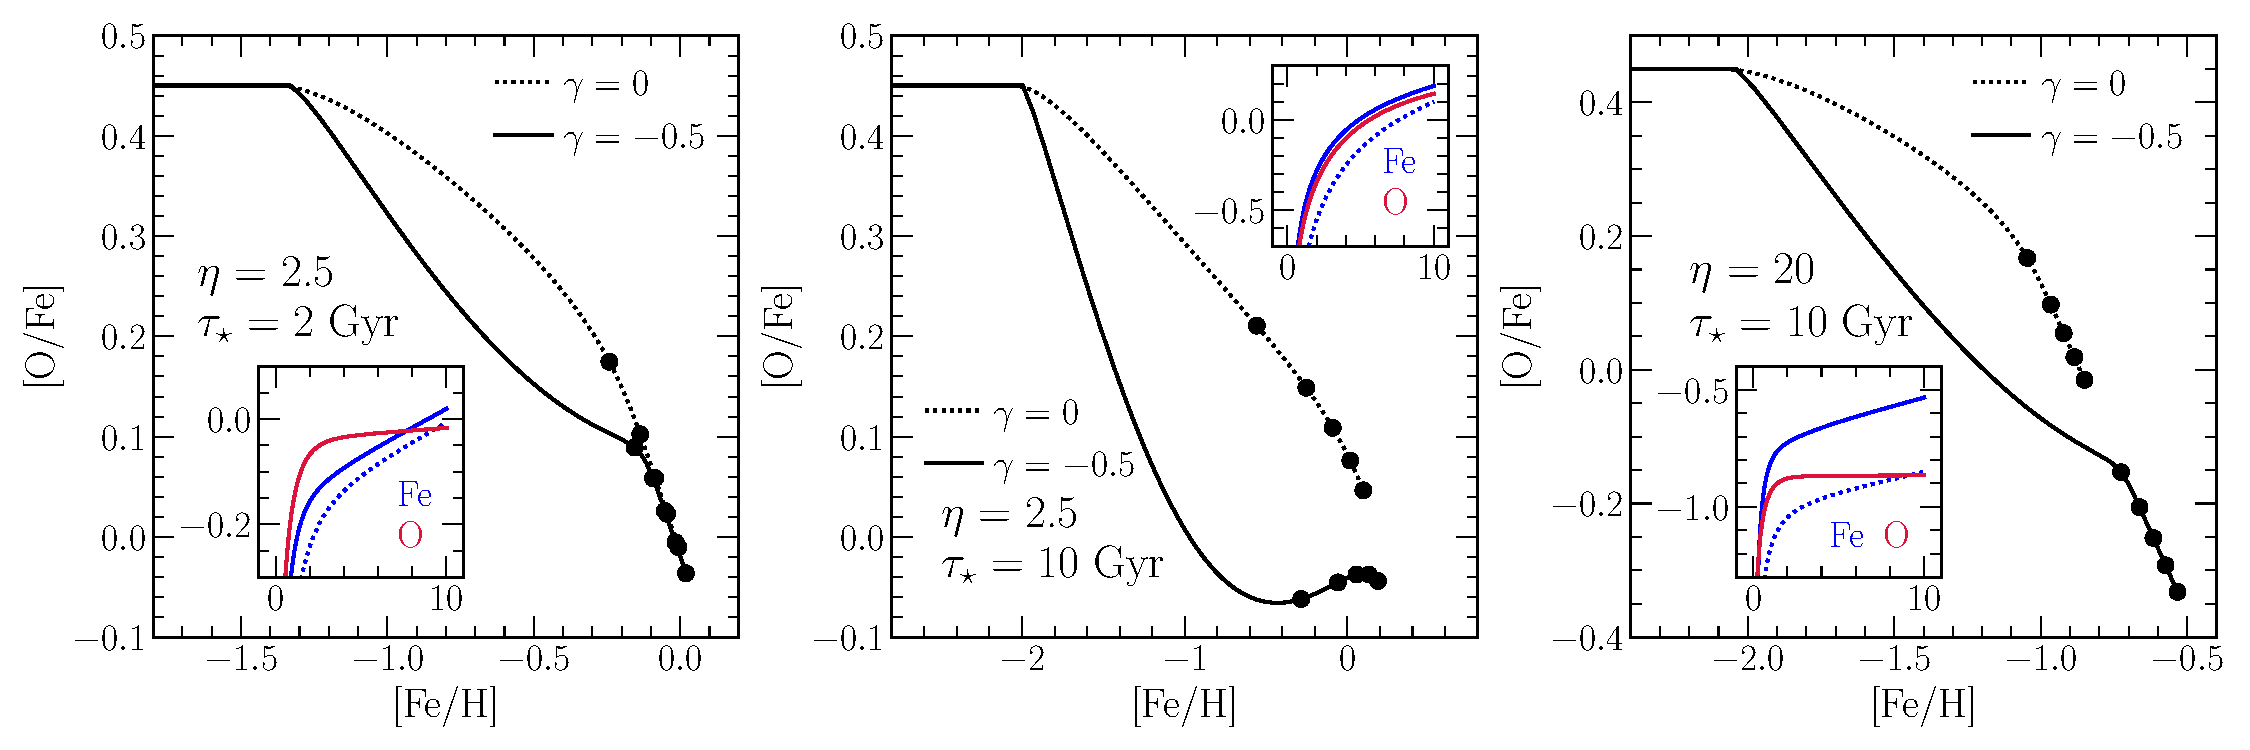
\includegraphics[scale = 0.46]{onezone_application.pdf}
\caption{
A comparison of one-zone galactic chemical evolution models based on
\citet[][for details, see their~\S~2]{Johnson2020} with ($\gamma = -0.5$,
solid) and without ($\gamma = 0$, dotted) metallicity-dependent SN Ia rates.
Tracks denote the O and Fe abundances in the interstellar medium parametrized
as a function of time with points marked at~$T = 2$, 4, 6, 8, and 10 Gyr.
Insets illustrate [O/H] and [Fe/H] as a function of time in Gyr for the
corresponding model.
We note on each panel the choice of the outflow mass-loading factor~$\eta$ and
the star formation efficiency timescale~$\tau_\star$.
}
\label{fig:onezone_app}
\end{figure*}

While empirical measurements of the specific SN Ia rate as a function of
stellar mass depend on the assumed SMF~\citep{Gandhi2022}, the host galaxy
mass distribution of observed events does not, making it a potentially more
observationally feasible diagnostic.
As noted in Fig.~\ref{fig:specia_metdep}, only dwarf galaxies are
significantly affected by a metallicity-dependent scaling of SN Ia rates due to
the shape of the MZR, so a~$\gamma \approx -0.5$ scaling should appear as an
enhanced SN Ia rate at the low-mass end of the distribution.
Although this empirical measurement does not depend on the SMF, our theoretical
prediction does because we must take into account the relative abundances of
galaxies of different stellar masses.
The observed rate in a bin of stellar mass can be expressed as the product
of the characteristic rate~$\dot{\text{N}}_\text{Ia}$ at a given stellar mass
and the integral of the SMF~$\Phi(\mstar)$ over the bin in stellar mass,
\begin{equation}
\dot{N}_\text{Ia,cosmic}(M_\star | \gamma) = \dot{N}_\text{Ia}(M_\star | \gamma)
\int_{M_\star}^{M_\star + dM_\star} \Phi(M_\star) dM_\star,
\label{eq:hostmassdist}
\end{equation}
where~$\dot{\text{N}}_\text{Ia}$ is the numerator of equation~\refp{eq:specia}.
We show this distribution in Fig.~\ref{fig:hostmassdist} for each combination
of~$\gamma = 0$ and~$-0.5$ and the~\citet{Bell2003} and~\citet{Baldry2012} SMFs,
normalizing to a maximum value of unity.
For untargeted surveys like ASAS-SN, equation~\refp{eq:hostmassdist} should
describe the observed host galaxy stellar mass distribution exactly, whereas
targeted surveys like the Lick Observatory SN Search~\citep[LOSS;][]{Li2000,
Filippenko2001} would need to correct for their target galaxy selection
criteria.
\par
Fig.~\ref{fig:hostmassdist} shows that galaxies with stellar masses of
$\mstar = 10^{10} - 10^{11}~\msun$ should dominate the SN Ia rate for all
choices of the SMF and~$\gamma$.
This peak rate simply represents the galaxies that dominate the stellar mass.
For a given choice of the SMF, $\gamma = -0.5$ increases the number of SNe Ia
at~$\mstar \approx 10^{7.2}~\msun$ by a factor of~$\sim$3 relative to
$\gamma = 0$.
However, Fig.~\ref{fig:hostmassdist} also shows that the enhancement is small
compared to the differences between the two SMFs.
% However, Fig.~\ref{fig:hostmassdist} indicates that this observed distribution
% is a considerably better diagnostic of the SMF itself as opposed to the
% metallicity dependence of SN Ia rates or lack thereof.
Between the peak and~$10^{7.2}~\msun$, the ~\citet{Bell2003} host mass
distribution drops by~$\sim$2.5 orders of magnitude while
that of~\citet{Baldry2012} drops by~$\sim$1.5 orders of magnitude.
This difference illustrates the need for precise knowledge of the
SMF to accurately determine the metallicity-dependence of SN Ia rates.
% Fig.~\ref{fig:hostmassdist} illustrates the need for precise knowledge of the
% SMF to accurately determine the metallicity-dependence of SN Ia rates.



% Nonetheless, once precise knowledge of the SMF -- independent of SN rates -- is
% available, this diagnostic could distinguish between different models for the
% metallicity dependence of SN Ia rates.

\end{document}
